% Project:  paper-comparison
% Type:     pre-print version
% Author:   Edoardo Costantini
% Created:  2022-08-29
% Modified: 2022-10-27

% Preamble ------------------------------------------------------------------- %

\documentclass[a4paper,doc,floatsintext,natbib]{apa6}\usepackage[]{graphicx}\usepackage[]{xcolor}
% maxwidth is the original width if it is less than linewidth
% otherwise use linewidth (to make sure the graphics do not exceed the margin)
\makeatletter
\def\maxwidth{ %
  \ifdim\Gin@nat@width>\linewidth
    \linewidth
  \else
    \Gin@nat@width
  \fi
}
\makeatother

\definecolor{fgcolor}{rgb}{0.345, 0.345, 0.345}
\newcommand{\hlnum}[1]{\textcolor[rgb]{0.686,0.059,0.569}{#1}}%
\newcommand{\hlstr}[1]{\textcolor[rgb]{0.192,0.494,0.8}{#1}}%
\newcommand{\hlcom}[1]{\textcolor[rgb]{0.678,0.584,0.686}{\textit{#1}}}%
\newcommand{\hlopt}[1]{\textcolor[rgb]{0,0,0}{#1}}%
\newcommand{\hlstd}[1]{\textcolor[rgb]{0.345,0.345,0.345}{#1}}%
\newcommand{\hlkwa}[1]{\textcolor[rgb]{0.161,0.373,0.58}{\textbf{#1}}}%
\newcommand{\hlkwb}[1]{\textcolor[rgb]{0.69,0.353,0.396}{#1}}%
\newcommand{\hlkwc}[1]{\textcolor[rgb]{0.333,0.667,0.333}{#1}}%
\newcommand{\hlkwd}[1]{\textcolor[rgb]{0.737,0.353,0.396}{\textbf{#1}}}%
\let\hlipl\hlkwb

\usepackage{framed}
\makeatletter
\newenvironment{kframe}{%
 \def\at@end@of@kframe{}%
 \ifinner\ifhmode%
  \def\at@end@of@kframe{\end{minipage}}%
  \begin{minipage}{\columnwidth}%
 \fi\fi%
 \def\FrameCommand##1{\hskip\@totalleftmargin \hskip-\fboxsep
 \colorbox{shadecolor}{##1}\hskip-\fboxsep
     % There is no \\@totalrightmargin, so:
     \hskip-\linewidth \hskip-\@totalleftmargin \hskip\columnwidth}%
 \MakeFramed {\advance\hsize-\width
   \@totalleftmargin\z@ \linewidth\hsize
   \@setminipage}}%
 {\par\unskip\endMakeFramed%
 \at@end@of@kframe}
\makeatother

\definecolor{shadecolor}{rgb}{.97, .97, .97}
\definecolor{messagecolor}{rgb}{0, 0, 0}
\definecolor{warningcolor}{rgb}{1, 0, 1}
\definecolor{errorcolor}{rgb}{1, 0, 0}
\newenvironment{knitrout}{}{} % an empty environment to be redefined in TeX

\usepackage{alltt}

% Packagaes
\usepackage[english]{babel}
\usepackage[utf8x]{inputenc}
\usepackage{amsmath}
\usepackage{bm}
\usepackage{graphicx}
\usepackage[colorinlistoftodos]{todonotes}
\usepackage[
	colorlinks,
	bookmarksopen,
	bookmarksnumbered,
	citecolor=red,
	urlcolor=red]{hyperref}	% automatic pdf outline and hyperlinks style
\usepackage{lineno} % for line numbering
\usepackage{color}
\usepackage{xcolor}			% for colors to track changes
\usepackage{placeins} 		% for FloatBarrier
\usepackage[normalem]{ulem} % for strikeout corrections
\usepackage{lineno} % for line numbering
\usepackage{tabularx}
\usepackage{adjustbox} % to make tables fit pages

% Macros
\renewcommand{\linenumberfont}{\tiny\color{gray}} % make linenum small and gray
\renewcommand{\thefootnote}{\arabic{footnote}}
\newcommand{\norm}[1]{\left\lVert#1\right\rVert} % for l2 norm in equations

% Paths (self-contained)
\newcommand{\pathBIB}{./bib}
\newcommand{\pathFIG}{./figures}

% Article information
\title{Paper title}
\shorttitle{Short title}
\twoauthors
	{Edoardo Costantini}
	{Author 2}
\twoaffiliations
	{Tilburg University, Department of Methodology and Statistics}
	{Utrecht University, Department of Methodology and Statistics}
\authornote{
  Corresponding author's contacts: \\
  e.costantini@tilburguniversity.edu; \\
  +31 **************
  }

% Abstract
\abstract{
This is some abstract.}

% Main Document -------------------------------------------------------------- %

\IfFileExists{upquote.sty}{\usepackage{upquote}}{}
\begin{document}
	\maketitle

    % Start section header numbering here
    \setcounter{secnumdepth}{3} % up to depth 3

    % Paper content
    
\section{Introduction}

    A captivating introduction is all you need.

\subsection{The power of knowing}

    Followed by a good description of previous studies \citep{collinsEtAl:2001}.
    
\section{Imputation methods and algorithms}\label{sec:methods}

	A selection of methods

\subsection{Method 1}

	Very cool method 1.

\subsection{Method 2}

	Very cool method 2.

\subsubsection{Aspect 1}

	Aspect 1

\subsubsection{Aspect 2}

	Aspect 2
    
\section{Simulation study 1}

	Why we did what we did.

\subsection{Simulation study procedure}

\subsubsection{Data generation}

	How we generated data	

\subsubsection{Missing data imposition}\label{sub-missing}

	How we imposed missing data	

\subsubsection{Imputation}

	Imputation models specification

\subsubsection{Analysis and comparison criteria}\label{criteria}

	Outcome measures

\subsection{Results}
	
	What results did we report

	% Load plots for this section


\subsubsection{Aspect 1}

	Here is a picture of what happened

	\begin{figure}
	\centering
\begin{knitrout}
\definecolor{shadecolor}{rgb}{0.969, 0.969, 0.969}\color{fgcolor}

{\centering 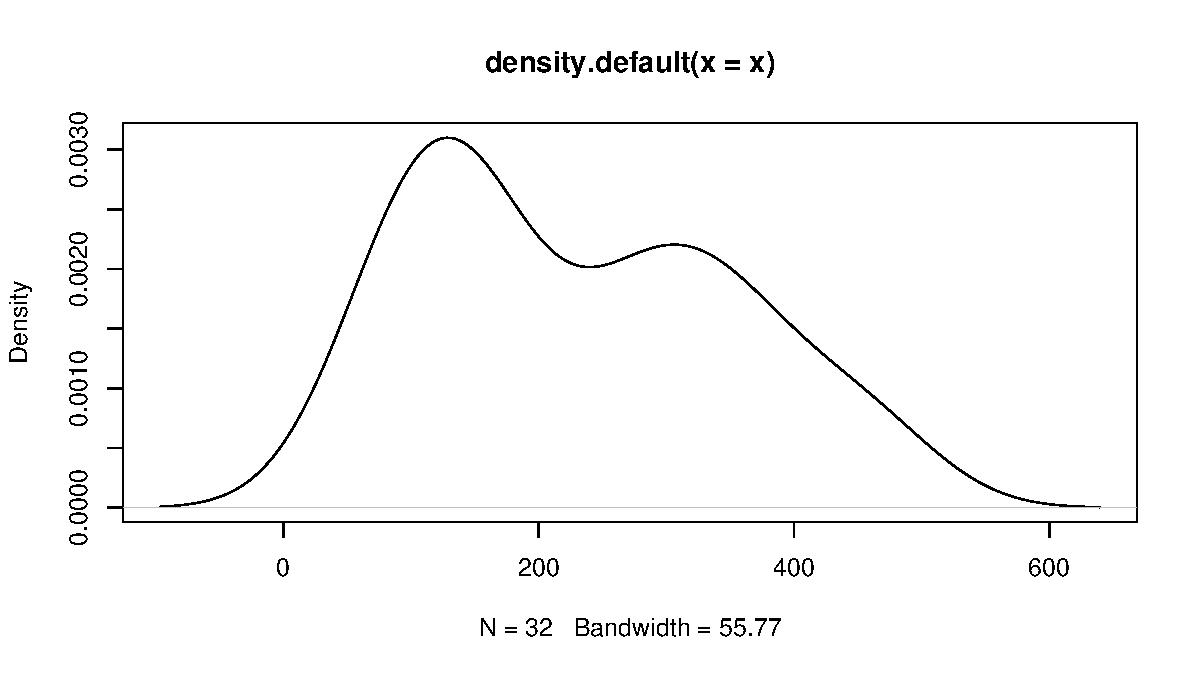
\includegraphics[width=\maxwidth]{figure/plot-pdf-1} 

}


\end{knitrout}
		\caption{\label{fig:dist} Some caption }
	\end{figure}

\subsubsection{Aspect 2}

	This is something else we found.
    
\section{Limitations and future directions}

	This is what's left to be done.
    
\section{Discussion}

\subsection{Methods that work well}

	Discuss it.

\subsection{Methods with mixed results}

	And discuss it.
    
    % Stop section header numbering here
    \setcounter{secnumdepth}{4}

    \section{Availability of data and materials}

    The data that support the findings of this study are available at [\url{https://some-url}].
    
    \section{Code availability}

    The code used for the study is available at the corresponding author's GitHub page: [\url{https://github.com/EdoardoCostantini/some-url}].
    Please read the README.md files for instructions on how to replicate the results.

    % References
    
\bibliographystyle{./style/asj}

\bibliography{
	\pathBIB/bibshelf
}

\end{document}
